\documentclass{article}
\usepackage{style}
\usepackage{amsmath}
\begin{document}
\maketitle
\part{Introducción}
\section{Neural Networks}

\subsection{Usos principales de las redes neuronales}

Se tienen 4 usos principales de las redes neuronales artificiales (RNA)
\begin{enumerate}
	\item Aproximación de sistemas (Modo regresor)
	\item Predicción de series de tiempo (Modo regresor)
	\item Control de Sistemas (Modo regresor)
	\item Clasificación de objetos (Modo Clasificador)
\end{enumerate}
\subsection{Aproximación de Sistemas}
Dado un sistema $f(t_i)$ del cuál se desconoce su modelo matemático, pero se cuenta con un conjunto de datos entrada-salida $(p, t)$ que representa su comportamiento. Se puede entrenar una RNA para que se comporte de manera similar a $f(t_i)$ en donde:\\\\
$t_i$ : Es la variable de tiempo\\
$p$ : Es la entrada (input)\\
$t$ : El valor deseado (target)\\

\subsection{Modelo Matemático}
Es una representación abstracta que aproxima al comportamiento de un fenómeno real, normalmente mediante un conjunto de ecuaciones.

\subsection{Ecuación}
Igualdad

\subsection{Datos input-output}
Es un conjunto de valores que muestrea mediante sensores el comportamiento dinámico del sistema en todo su rango de funcionamiento

\subsection{Buena Interpolación}
Se llama generación de conocimiento

\subsection{Mala Interpolación}
Se le llama sobrentendimiento

\textbf{LA RED EN MODO REGRESIÓN FUNCIONA COMO UN INTERPOLADOR}

\subsection{Extrapolar}
Pronosticar o predecir, se requieren RNA's recurrentes.

\subsection{Diagrama General}
\begin{figure}[h]
	\caption{Diagrama General}
	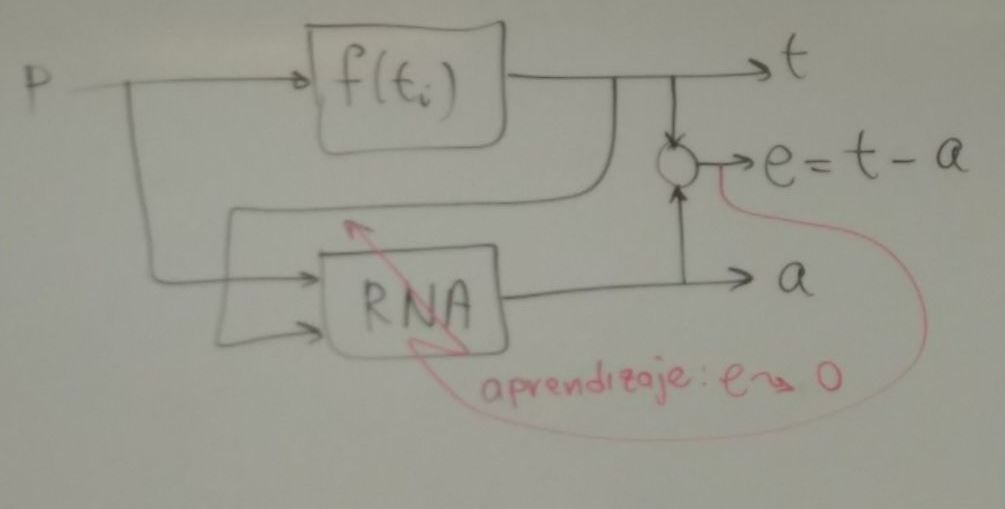
\includegraphics[scale=0.6]{modeloGeneralRn}
\end{figure}

\section{Tipos de Aprendizaje}
\subsection{Aprendizaje Supervisado}
Es aquel en el que se cuenta con ejemplos que contienen valores deseados(target) para llevar a cabo el ajuste de los parámetros de la RNA. En este caso se cuenta con un conjunto de datos$(p, t)$;

\subsection{Aprendizaje no Supervisado}
No se cuenta con ejemplos que contengan valores deseados. Sin embargo, existen diversos algoritmos en esta clasificación que se usan para analizar y extraer información valiosa de una fenómeno, por ejemplo, el algoritmo $k-medias$ recibe como entrada un conjunto de datos y un valor $k$ que representa el número de clases en los que se desea separar a dicho conjunto. Dependiendo del valor de $k$ el usuario podrá analizar de diferentes maneras el fenómeno.

\section{Predicción de Series de tiempo}
Dada una serie de tiempo que representa un fenómeno físico, existe un tiempo especial de RNA que es capaz de pronosticar valores futuros, es decir, realiza la correcta extrapolación de datos. Para esta tarea se hace uso de las RNA's recurrrentes.
\begin{figure}
	\centering
	\caption{Ejemplo de extrapolación}
	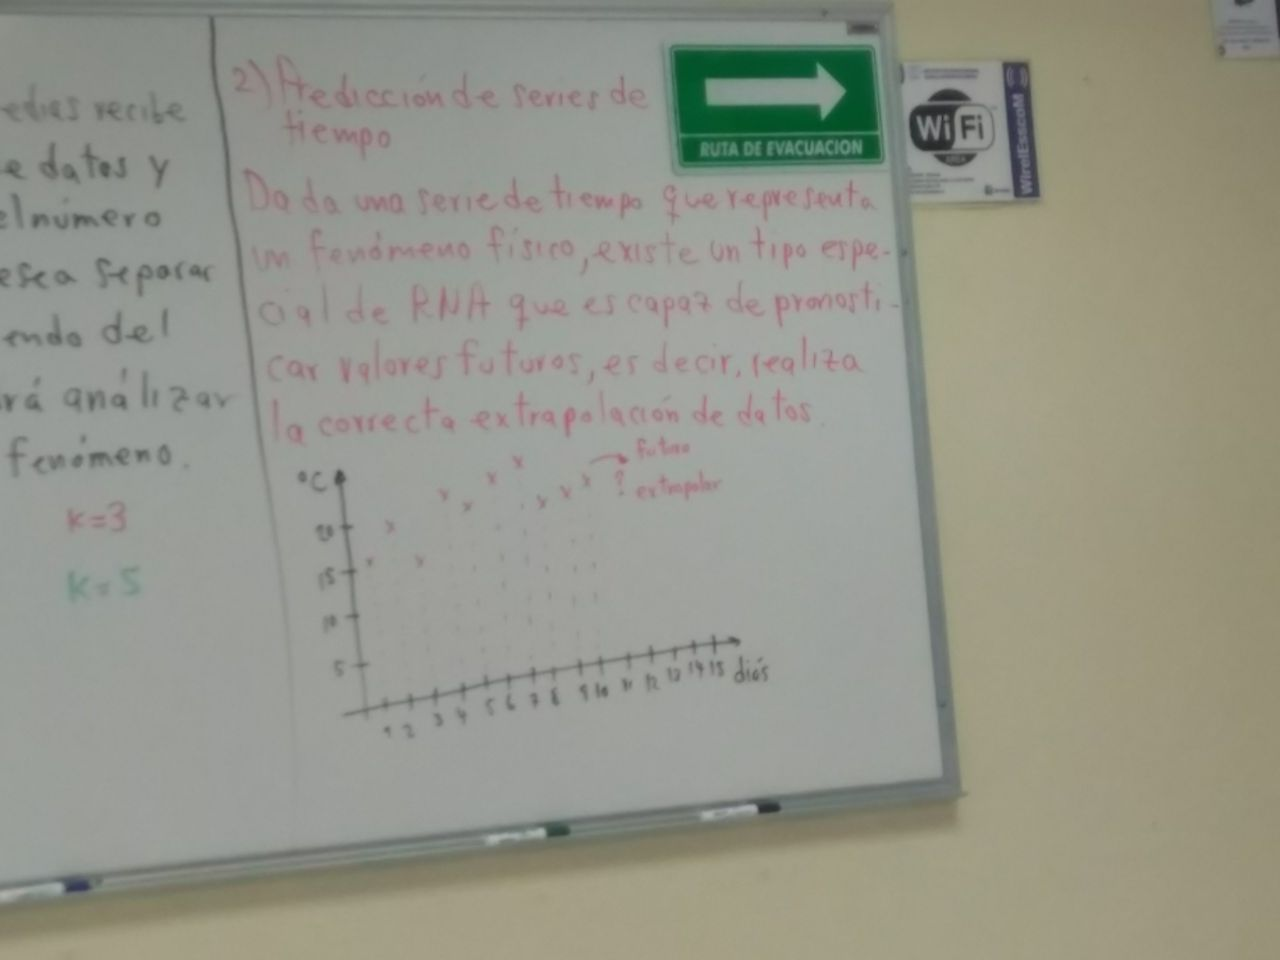
\includegraphics[scale=.4]{exampleTime}	
\end{figure}

\begin{figure}
	\centering
	\caption{Red Feed Foward}
	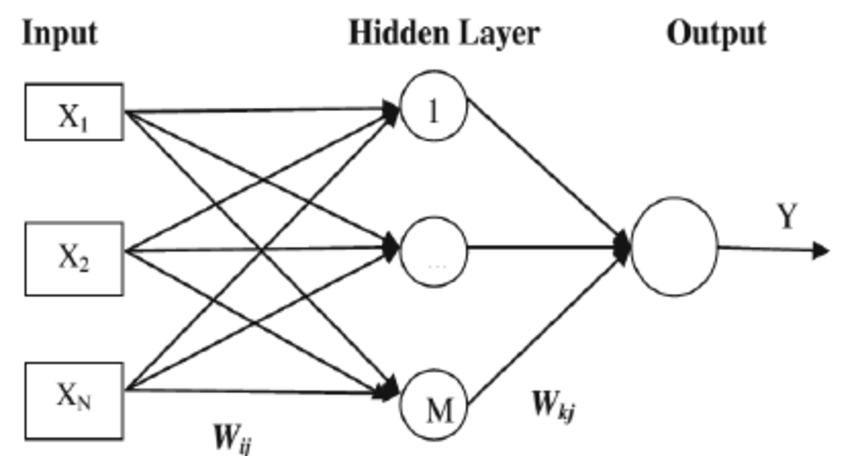
\includegraphics[scale=.5]{feedFowardExample}	
\end{figure}

\begin{figure}
	\centering
	\caption{Red Recurrente}
	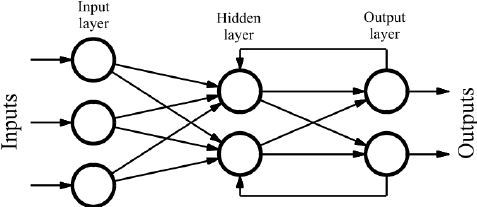
\includegraphics[scale=.8]{recurrentExample}	
\end{figure}

\begin{figure}
	\centering
	\caption{Red Recurrente con bloques recurrentes}
	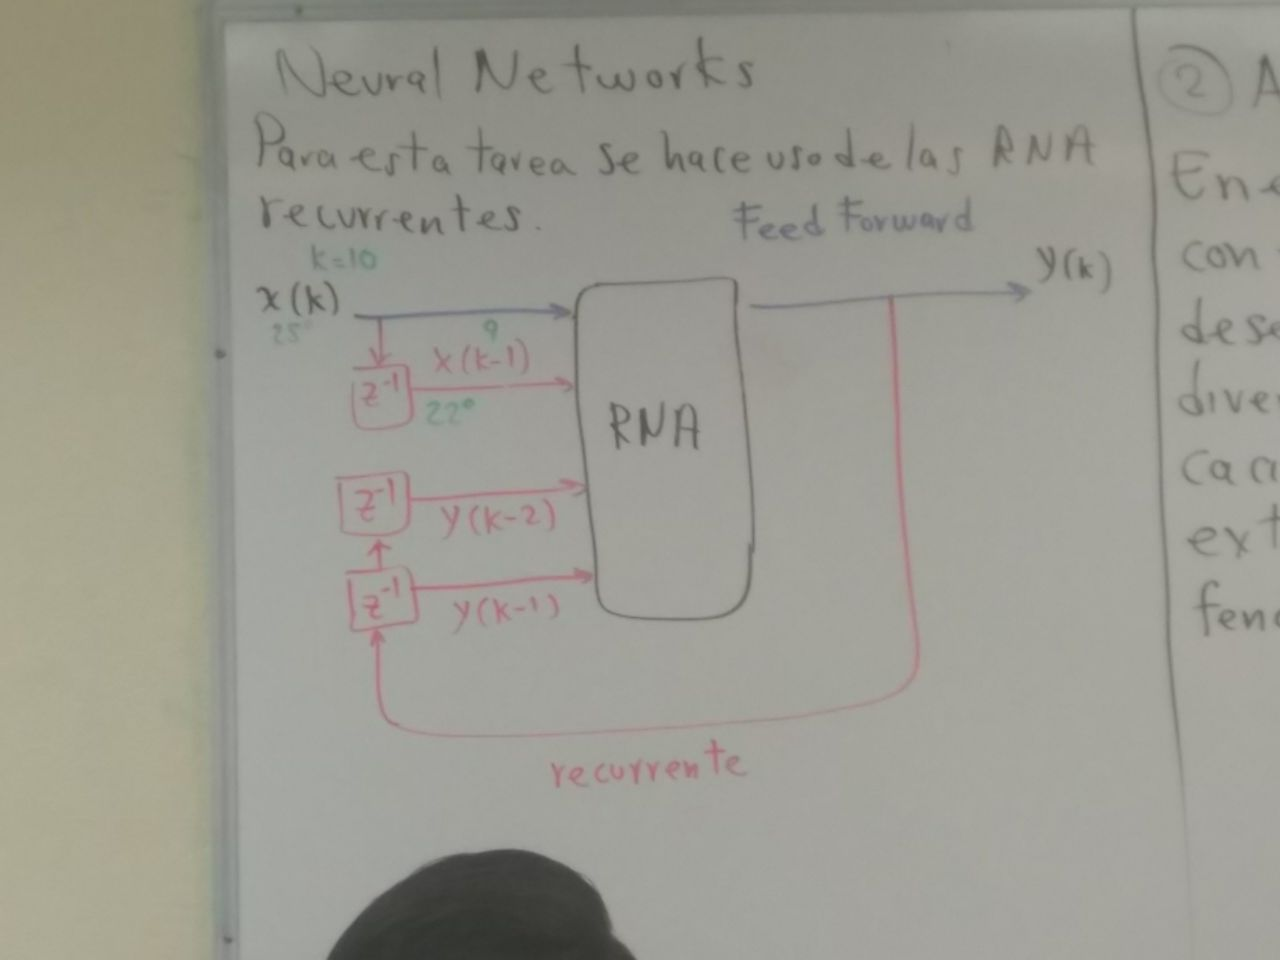
\includegraphics[scale=.37]{recurrentExample2}	
\end{figure}

\section{Control de Sistemas}
Dado un sistema $f(t)$ se requiere modificar su comportamiento para que sea estable. En esta aplicación se usa una RNA para aproximar a $f(t)$ y una RNA para diseñar un controlador.

\begin{figure}
	\centering
	\caption{System Control Example}
	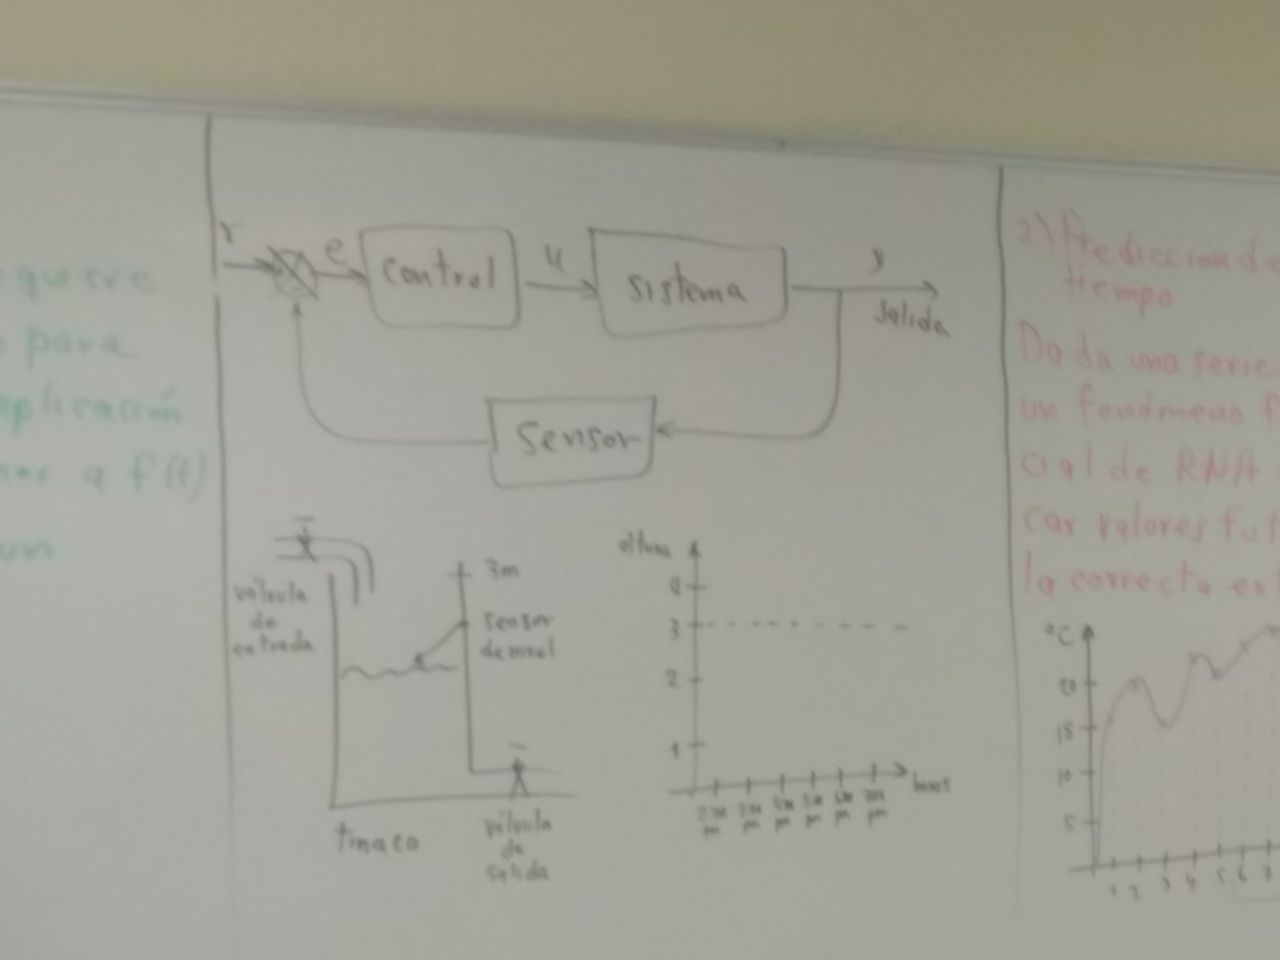
\includegraphics[scale=.37]{systemControlExample1}	
\end{figure}

\part{Aplicaciones de la RNA}
\section{Reporte de Práctica}
\begin{enumerate}
	\item Intro
	\item Metodología
	\item Pseudo código
	\item Resultados(Discusión)
	\item Conclusiones
	\item Referencias(mínimo 2)
\end{enumerate}
\section{Clasificación de Objetos}
Consiste en tener una adecuada separación de un conjunto de objetos mediante una función de semejanza.
\begin{enumerate}
	\item Clasificación supervisada:\\
	Aquí se cuenta con un conjunto de objetos y se conoce a que clase pertenence cada uno de ellos.\\
	Una RNA en modo clasificador puede usar una o más salidas para represtnar a que calse considera que un dato de entrada pertenece.\\
	Aquí tenemos targets ya que tenemos un conjunto de clases a las que este se puede etiquetar.\\
	Las redes pueden ser entrenadad no supervisadamente y supervisadamente\\
	Ejemplos:
	\begin{itemize}
		\item \begin{figure}[h!]
			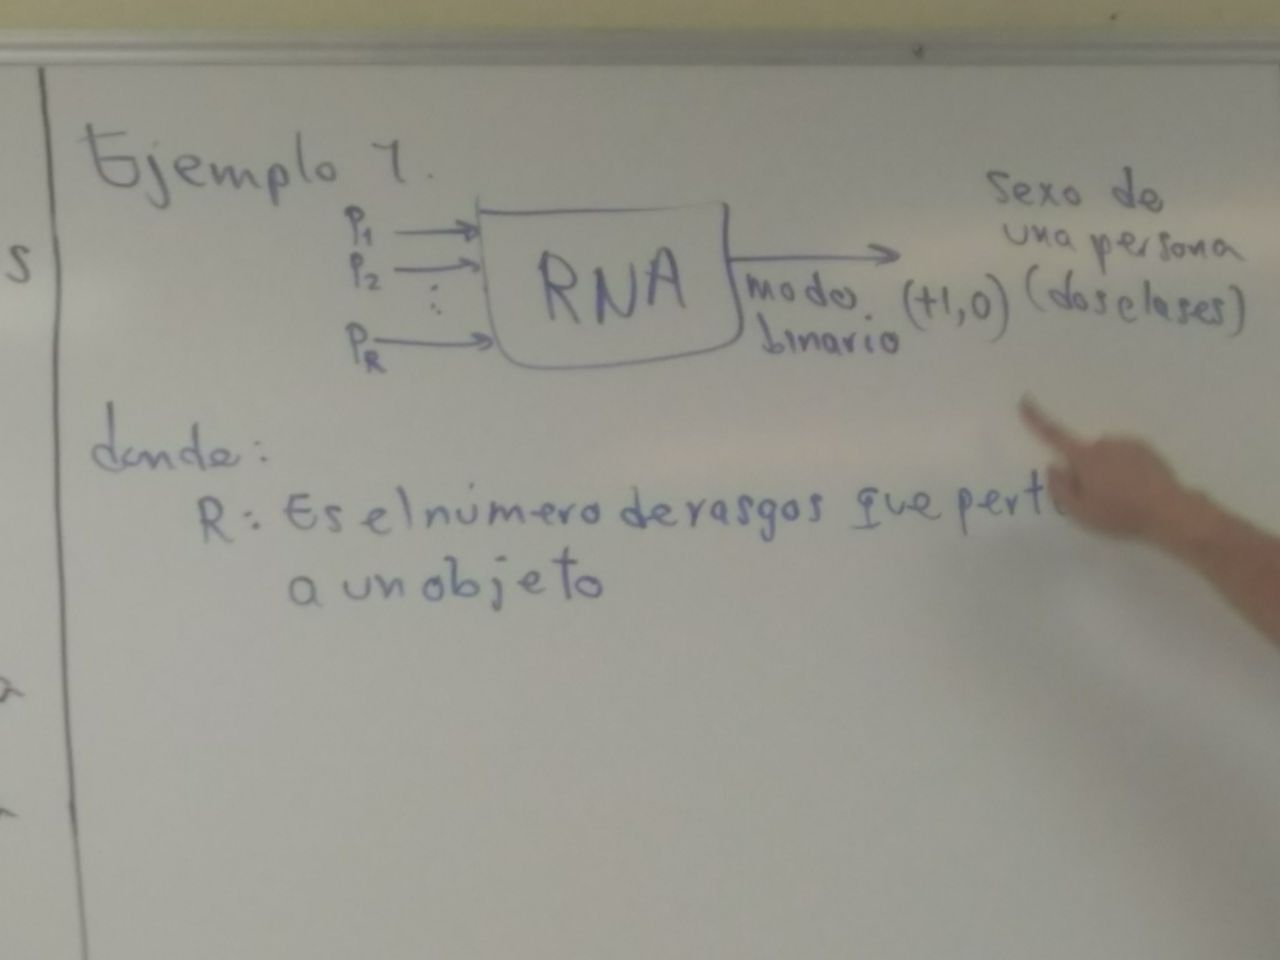
\includegraphics[scale=.2]{appEx1}
		\end{figure}
		\item \begin{figure}[h!]
			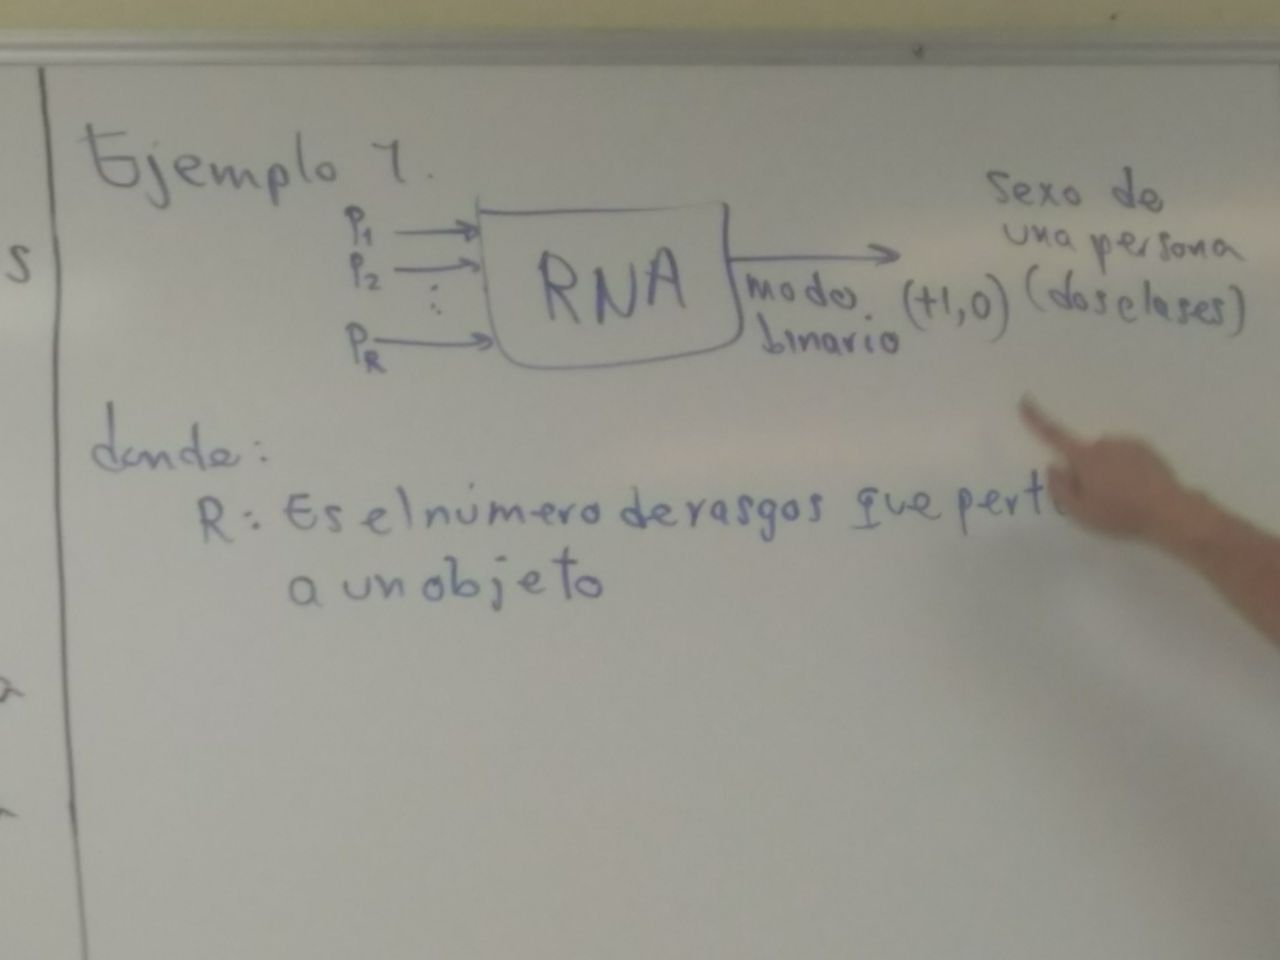
\includegraphics[scale=.2]{appEx2}
		\end{figure}
	\end{itemize}

\end{enumerate}
\section{Neurona Biológica}
Los sistemas biolgcos son tan complejos que se han convertido en una excelente fuente de inspiración para diseñar sistemas artificiales, que emulen algunas de sus características, entre ellas se encuentras las siguientes
\begin{enumerate}
	\item No siempre requieren de módulos de referencia (targets)
	\item Se desempeñan exitosamente ante incertidumbres
	\item Se adaptan fácilmente a nuevos ambientes
	\item Pueden Procesar información de diversas fuentes en forma simultánea
\end{enumerate}
Dado que las RNA nacieron de los elementos básicos de una neurona biológica, es bioinspirada.\\
Los componentes básicos de una neurona biológica son:\\
\begin{figure}[h!]
	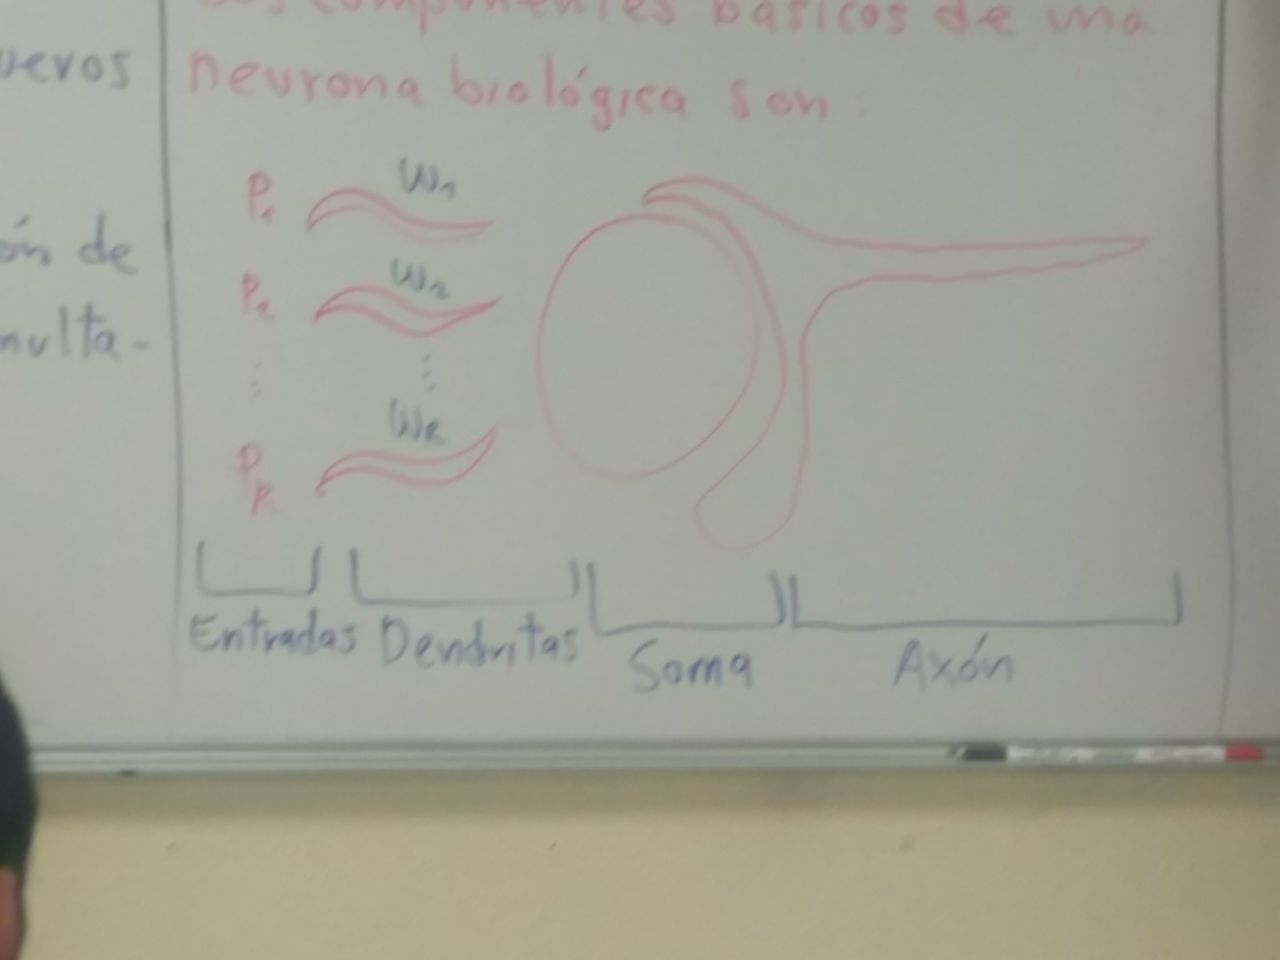
\includegraphics[scale=.20]{bioNeuron}
\end{figure}\\
donde:\\
$P_1,\ldots,P_r$: Son Entradas\\
$W_1, \ldots, W_r$: Son los pesos sinápticos\\
Los pesos sinápticos se usan para indicar el nivel de importancia de cada una de las conexiones para una tarea particular.\\
El soma se encarga de acumular energía y determinar cuando se generará una señal de salida.\\
\textbf{Nota: Para un target o tarea deseada, aprendizaje es buescar un conjutno de $W_1$ a $W_r$ tales que la salida de la red desea igual al target, para todos los datos del conjutno de entramiento}
\part{Arquitecturas de Redes}
\section{Notación}
\begin{itemize}
	\item Valores escalaras: minúsculas
	\item Valores vectoriales: Mayúsculas
\end{itemize}
\section{Modelo de neurona con una entrada}
\begin{figure}[h!]
	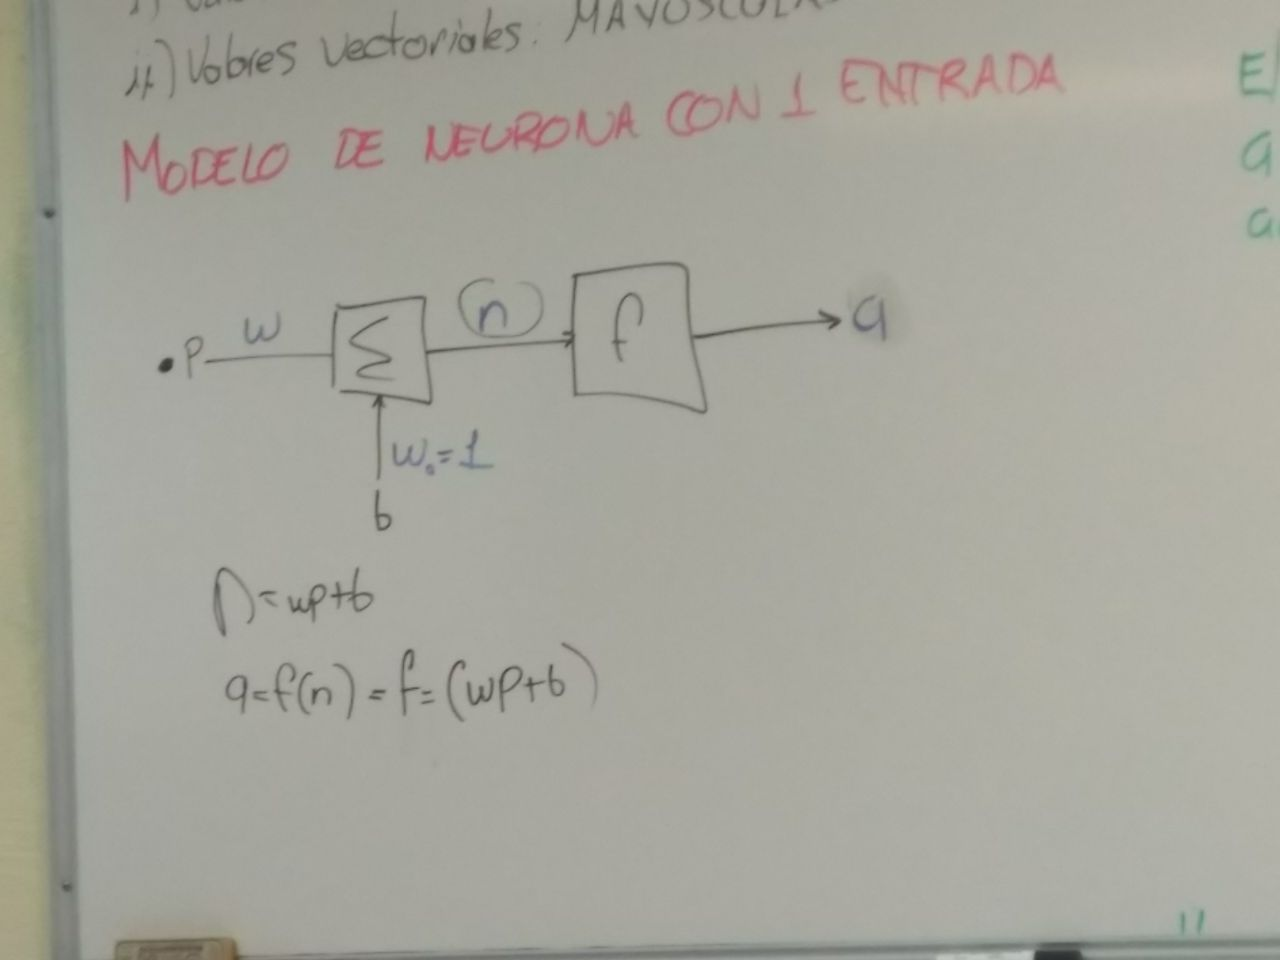
\includegraphics[scale=.3]{mculloc1}
\end{figure}
El bias es una entrada artificial que por definición tendrá siempre un peso sináptico de 1.\\
El bias como parámetro extra, le permite a la red resolver problemas más complejos, aunque existen RNA sin bias.\\
\newpage
Ejemplo:\\
Siendo p=2, w=3 y b=-1.5, sustituya en el modelo de la neurona con 1 entrada.\\
$a = f(4.5)$
\section{Neurona con múltiples entradas}
Típicamente, para resolver un problema, una neurona tiene más de una entrada. Estas se representan como $p_1, p_2, p_3, \ldots p_r$ y a cada una le corresponde un peso sináptico $w_{11}, w_{12}, \ldots, w_{1r}$\\
\begin{figure}[h!]
	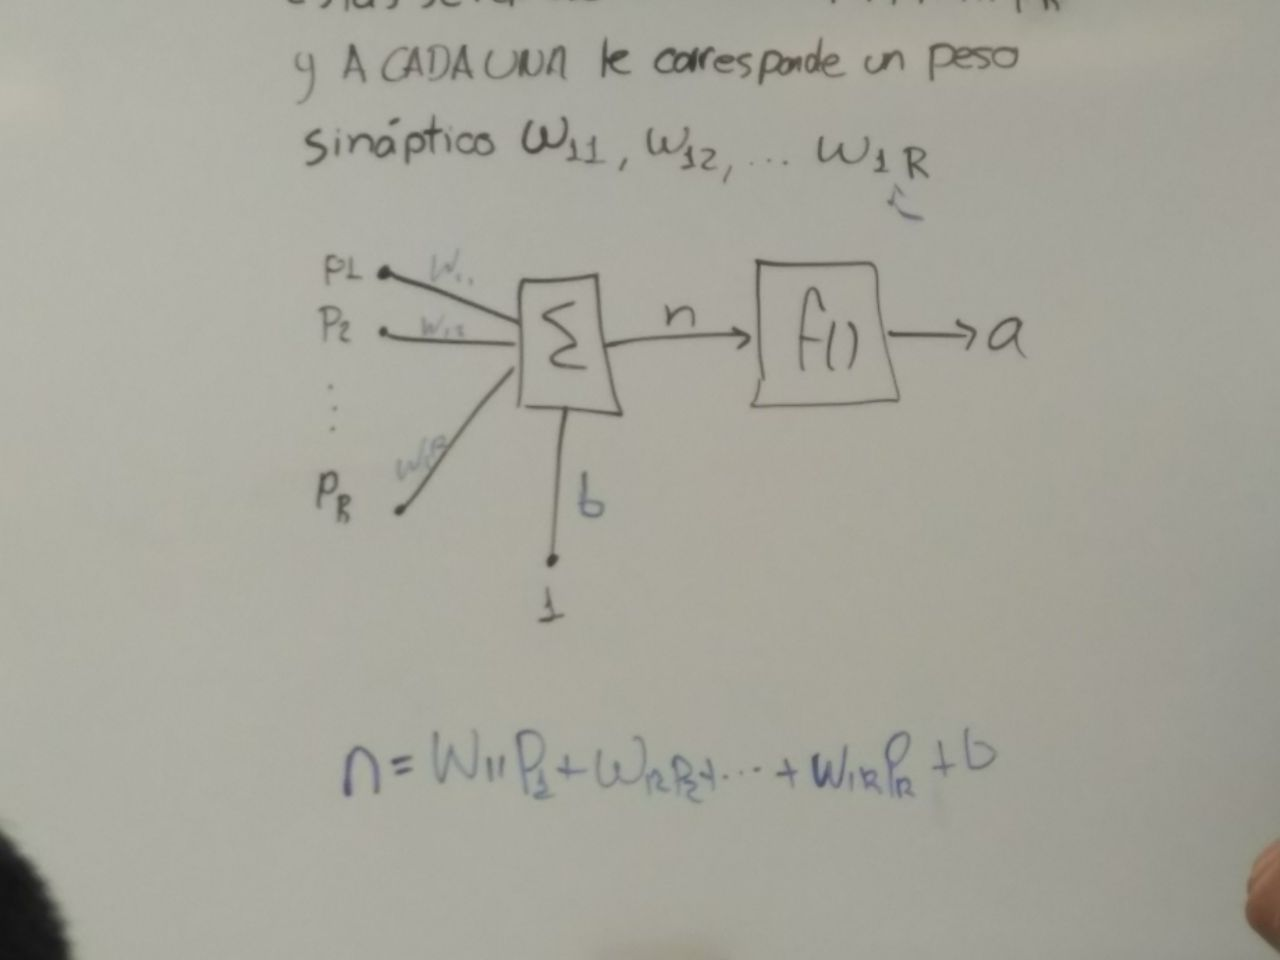
\includegraphics[scale=.3]{nneuron}
\end{figure}\\
En forma matricial, se puede expresar:\\
$n = W*P + b$\\
Donde n es un escalar\\
W es una matriz de [1Xr]\\
P es una matriz de [rx1]\\
b es una escalar\\
R es el número de entradas\\
1 es el número de neuronas\\

Finalmente, la salida de la red es:\\
$a = f(WP + b)$\\
Nota:\\
Para este caso particular, la matriz de pesos W es un vecotr fila, ya que representa el número de neuronas en cada capa de la RNA
\subsection{Índices de la matriz W}
Durante el curso, se utilizó la siguiente convención para los índices de la matriz de pesos:\\
\begin{enumerate}
	\item El primer índice, se refiere a la Neurona a la que llega a la conexión.
	\item El segundo índice indica el número  de la \textbf{Fuente} de la que proviene el dato
\end{enumerate}
\subsection{Representación Gráfica matricial}
\begin{figure}[h!]
	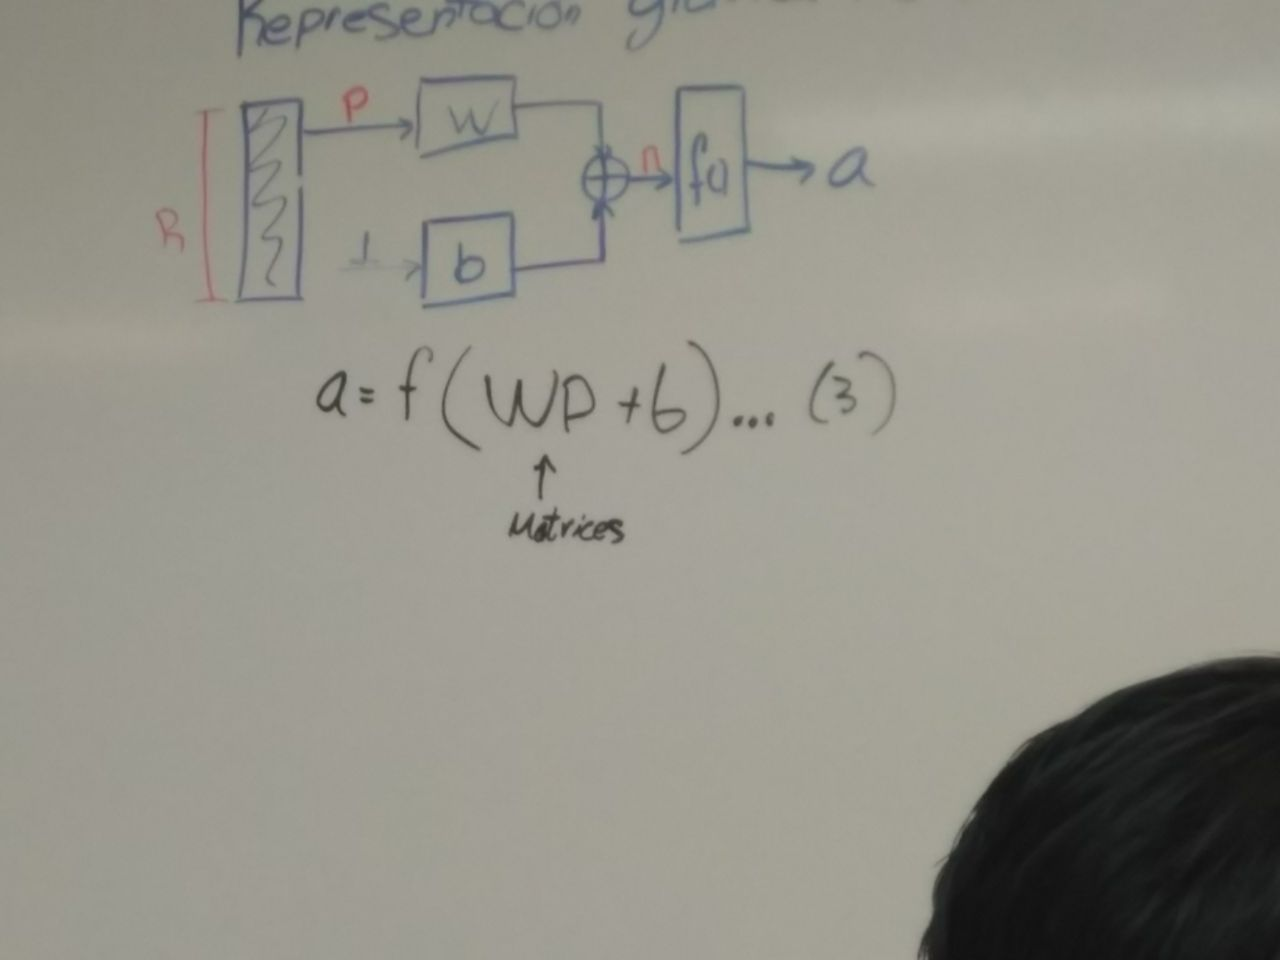
\includegraphics[scale=.3]{matrixgrep}
\end{figure}
\newpage
\section{Múltiples neuronas en Paralelo con múltiples entradas(Una capa)}
\begin{figure}[h!]
	\centering
	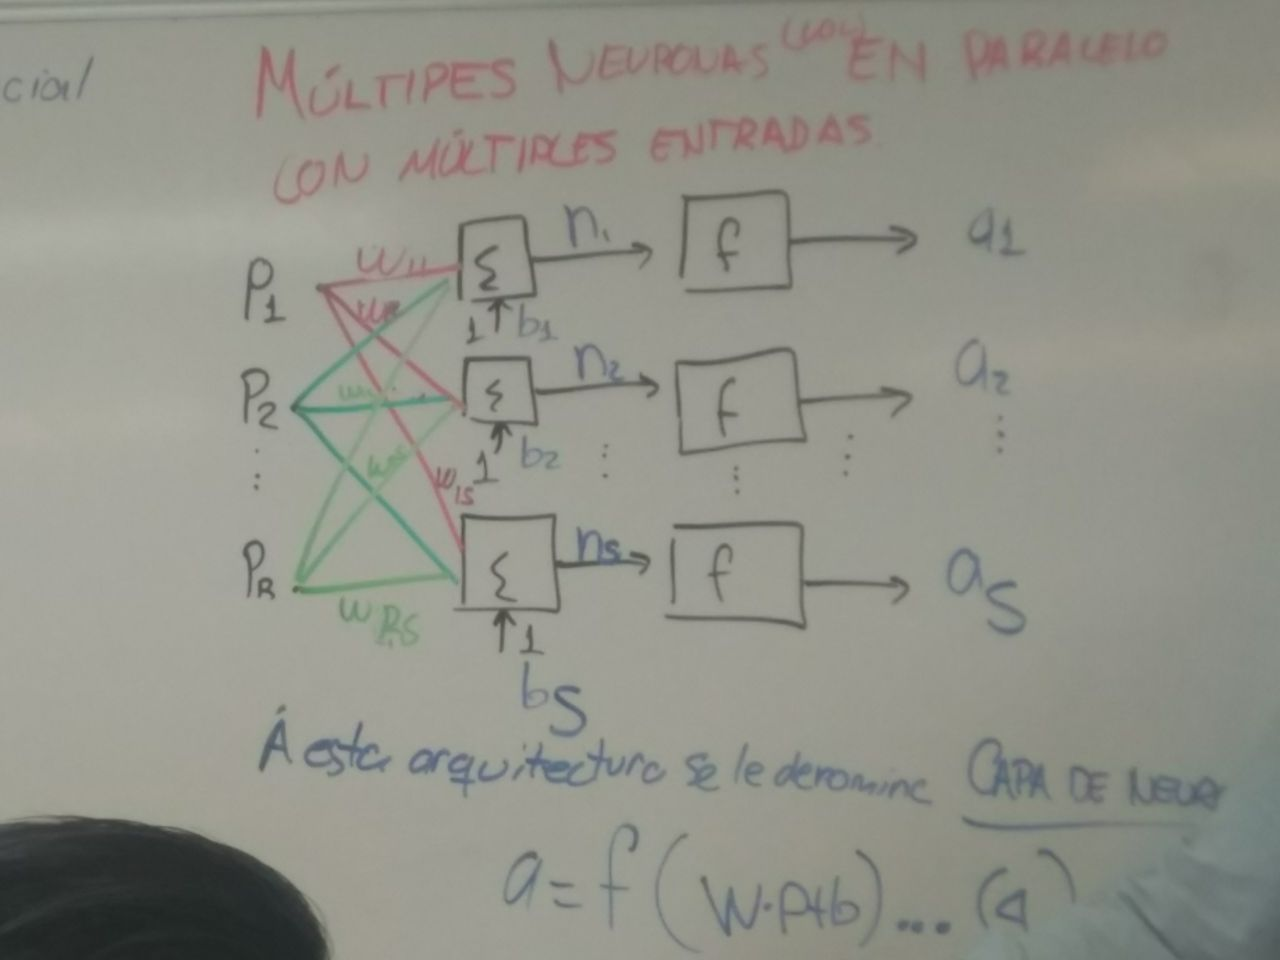
\includegraphics[scale=.3]{layersmodel}
	\caption{Arquitectura  ``Capa de neuronas''}
\end{figure}
$a = f(w*p+b)$\\
donde las dimensiones de w son: SxR\\
las dimensiones de P son: RxS\\
las dimensiones de b son Sx1
\newpage
\subsection{Diagrama Simplificado}
\begin{figure}[h!]
	\centering
	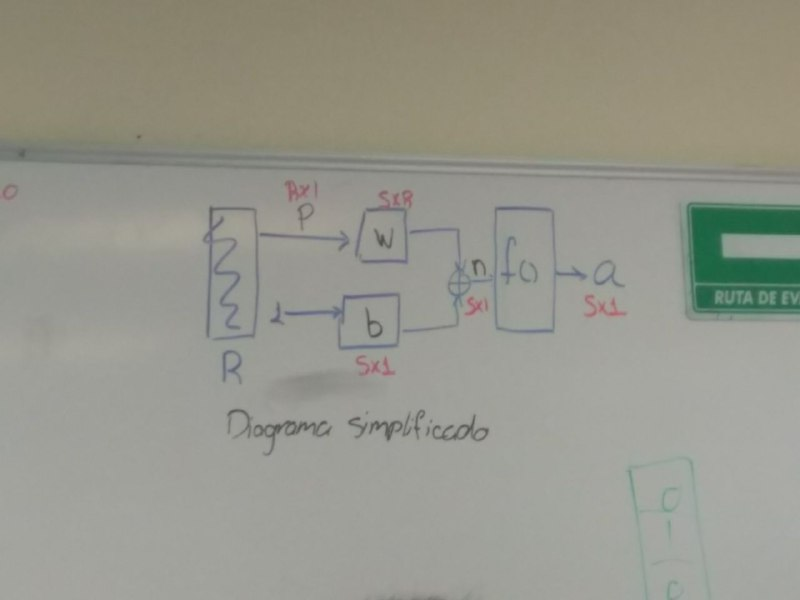
\includegraphics[scale=.3]{simpdiagram}
	\caption{Arquitectura  ``Capa de neuronas'' en diagrama simplificado}
\end{figure}
\subsection{Ejemplo con s = 1}
\begin{figure}[h!]
	\centering
	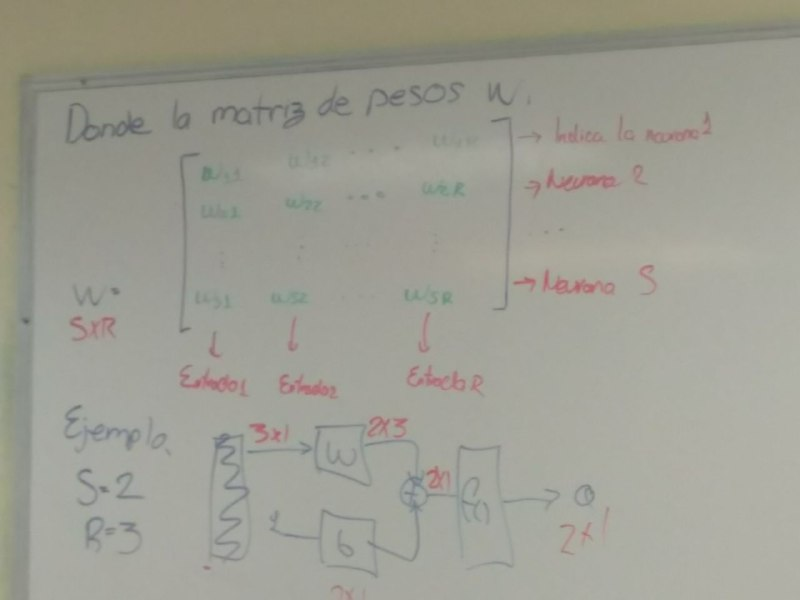
\includegraphics[scale=.3]{matrixejpar}
	\caption{Matriz de pesos $W_i$}
\end{figure}
\subsubsection{Nota acerca de las capas}
Algunos autores llaman al vector de entrada P ``Capa de entrada''.\\
Sin embargo, como en ella no se llevan a cabo operaciones, durante el curso \textbf{NO LO HAREMOS}
\begin{itemize}
	\item Capas Ocultas: Se les llama así porque no tiene contacto con el exterior(Hidden Layers)
	\item Capa de Salida: Es aquella que entrega el resultado
\end{itemize}

\section{Multiples Capas de Neuronas}
Ahora se considerará una RNA con varias entradas y múltiples capas. Cada capa tiene su propia matriz de pesos $w$, vector de bias $b$ y vector de salida $a$. Para distinguir entre cada capa, agregamos un superíndice o la variable.
$$ a^1 = f^1(w_s^1p_r^1b_s^1)$$ $$a^2=f^2(w^2a^1+b_s^2)$$
\begin{figure}[h!]
	\centering
	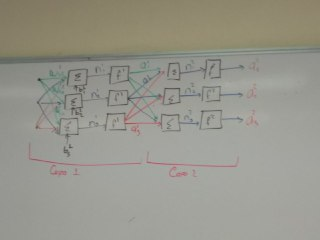
\includegraphics[scale=1]{rainbowmodel}
	\caption{Modelo Arcoiris}
\end{figure}
\begin{figure}[h!]
	\centering
	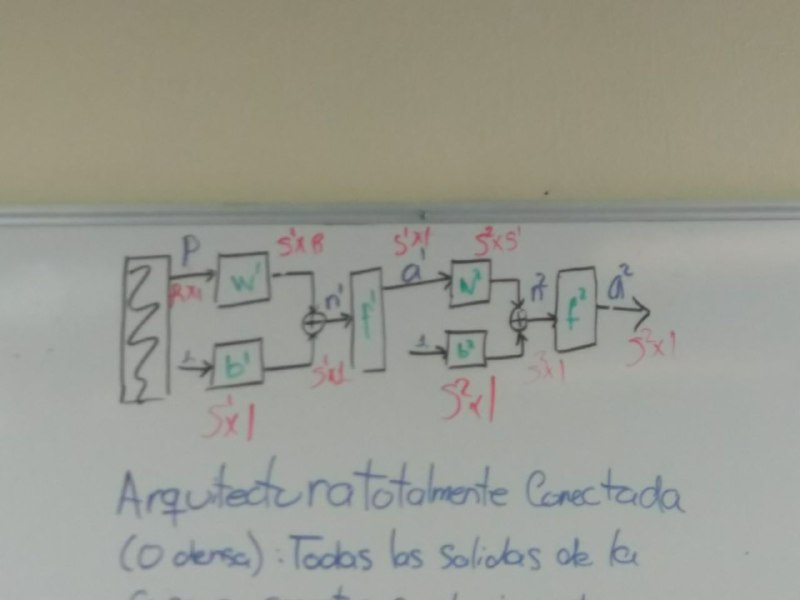
\includegraphics[scale=.4]{rainbowsingle}
	\caption{Capa del modelo arcoiris}
\end{figure}
\newpage
\section{Arquitectura totalmente conectada (O densa)}
$$ a^2 = f^2[w^2f^1(w^1p+b^1)+b^2] $$
Para representar una arquitectura multicapa, (MLP-Multilayer-Perceptron) se utiliza notación:$$ [R\ S^1\ S^2 \ S^3 \dots\ S^m]$$
Donde:\\
R: Es el número de entradas\\
M: Es el número de capas.\\
$S^1 \dots\ S^m$: El número de neuronas en cada capa
\subsection{Ejemplo}
[4 2 5 1]\newline
[$P$] = 4x1\newline
[$w^1$] = 2x4\newline
[$w^2$] = 5x2\newline
[$w^3$] = 1x5\newline
[$b^1$] = 2x1\newline
[$b^2$] = 5x1\newline
[$b^3$] = 1x1
\section{Multilayer Perceptron (MLP)}
La arquitectura mínima de un MLP es [$R$ $S^1$ $S^2$], pero ¿Cómo seleccionas la arquitectura?\\
Debemos partir de las especificaciones del problema, ello nos permite definir lo siguiente:
\begin{enumerate}
	\item El número de entradas (R) al MLP es igual al número de rasgos o variables usados en el problema
	\item El número de neuronas en la capa de salida es igual al número de clases definida en el problema
	\item El tipo de función de activación depende de las consideraciones del problema
	\item En cuanto al número de capas ocultas y al número de neuronas en cada una de ellas, sigue siendo un problema abierto
\end{enumerate}
\subsection{Ejemplo}
Determinemos la arquitectura que clasifique los siguientes objetos en 2 clases\\
\diagram{$O_1=$}{$R_1$\\$R_2$\\$R_3$} \diagram{$O_2=$}{$R_1$\\$R_2$\\$R_3$} \diagram{$O_3=$}{$R_1$\\$R_2$\\$R_3$} \diagram{$O_4=$}{$R_1$\\$R_2$\\$R_3$}\newline
[3 \hspace{10px} 2]
\subsection{Uso del MLP}
\begin{itemize}
	\item Para problemas de aproximación de señales, es común pensar que la dimensión de la señal de entrada Sea R=1. Se usan 1 o 2 capas ocultas y una neurona de la capa de salida
\end{itemize}
\section{Funciones de transferencia}
\subsection{Función Hardlim}
Esta función genera un cero como salida si n es menor a cero y uno si el valor de n es mayor o igual a cero($n \ge 0$).\\
Esta función se usa para crear neuronas capaces de clasificarlas entradas en dos clases.
\begin{figure}[h!]
	\centering
	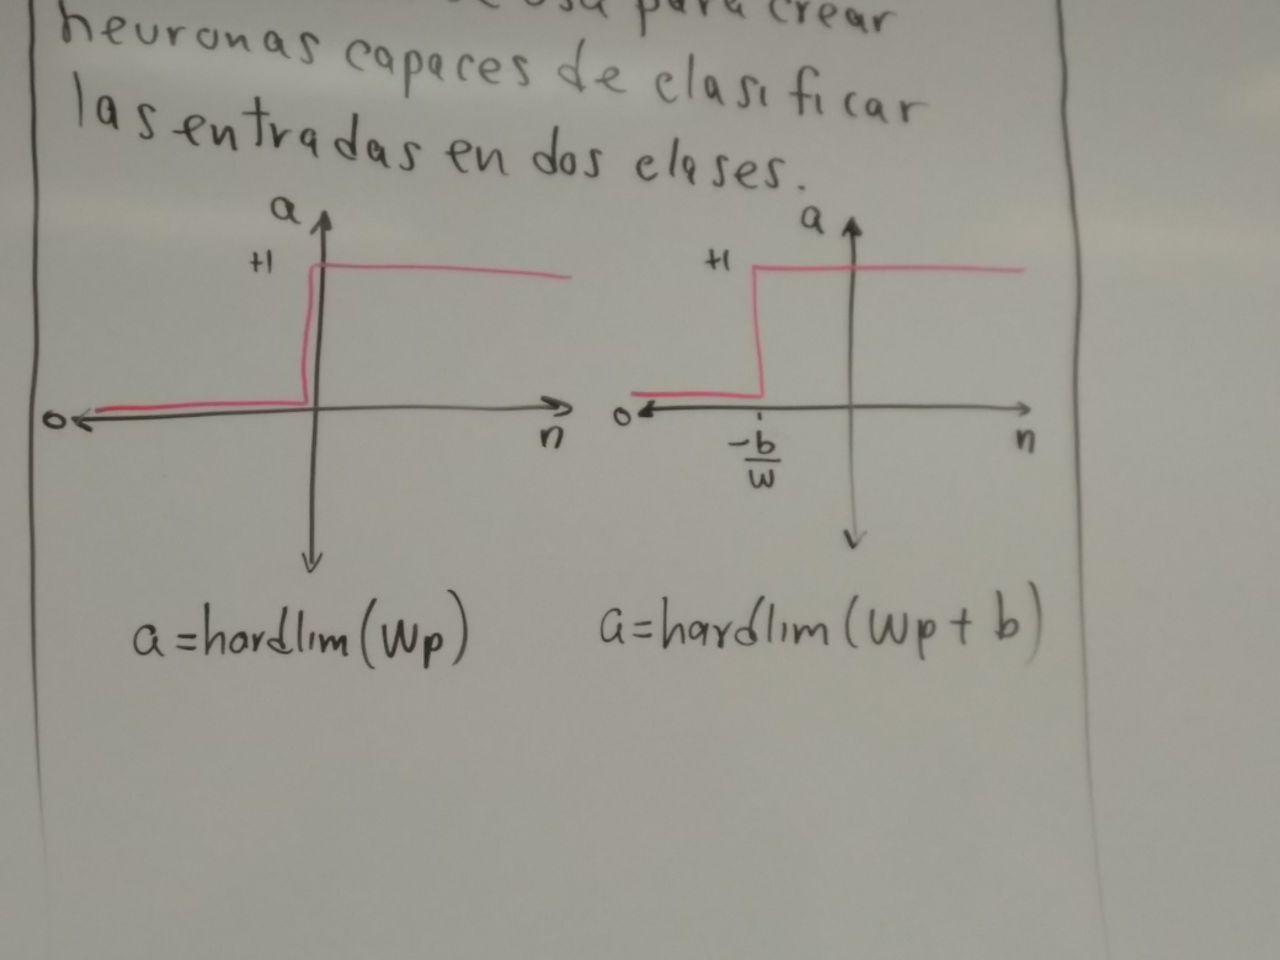
\includegraphics[scale=.2]{hardlim}
	\caption{Función HardLim}
\end{figure}
\newpage
\subsection{Función Lineal}
En esta función la salida es igual a la entrada
$$a = n$$\\
Este tipo de función se usa para trareas de regresión(aproximación de señales), por ejemplo la red ADALINE
\begin{figure}[h!]
	\centering
	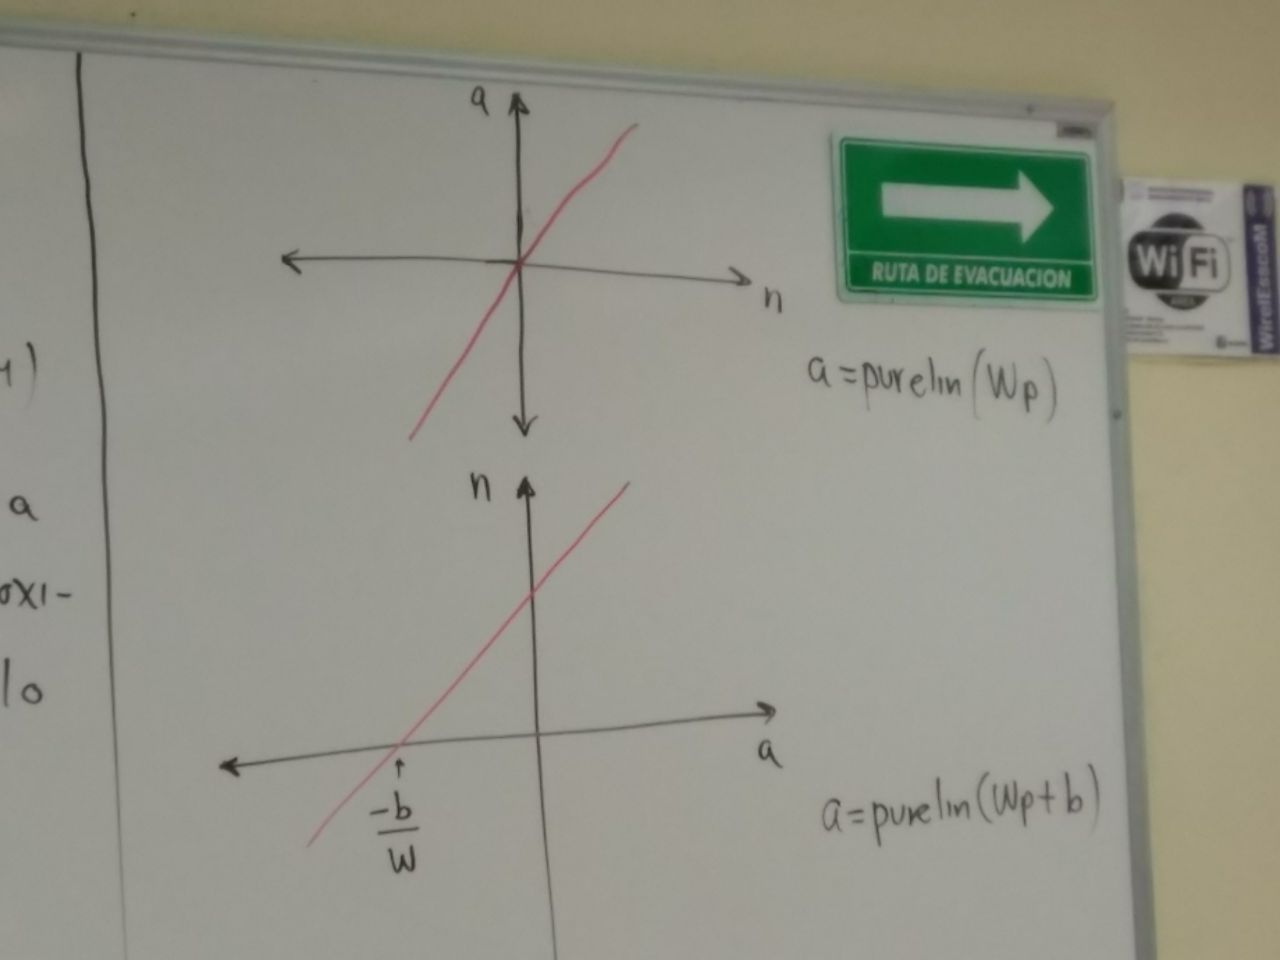
\includegraphics[scale=.2]{purelim}
	\caption{Función PureLim}
\end{figure}
\subsubsection{Ejemplo}
Aproximación de señales\\
\begin{figure}[h!]
	\centering
	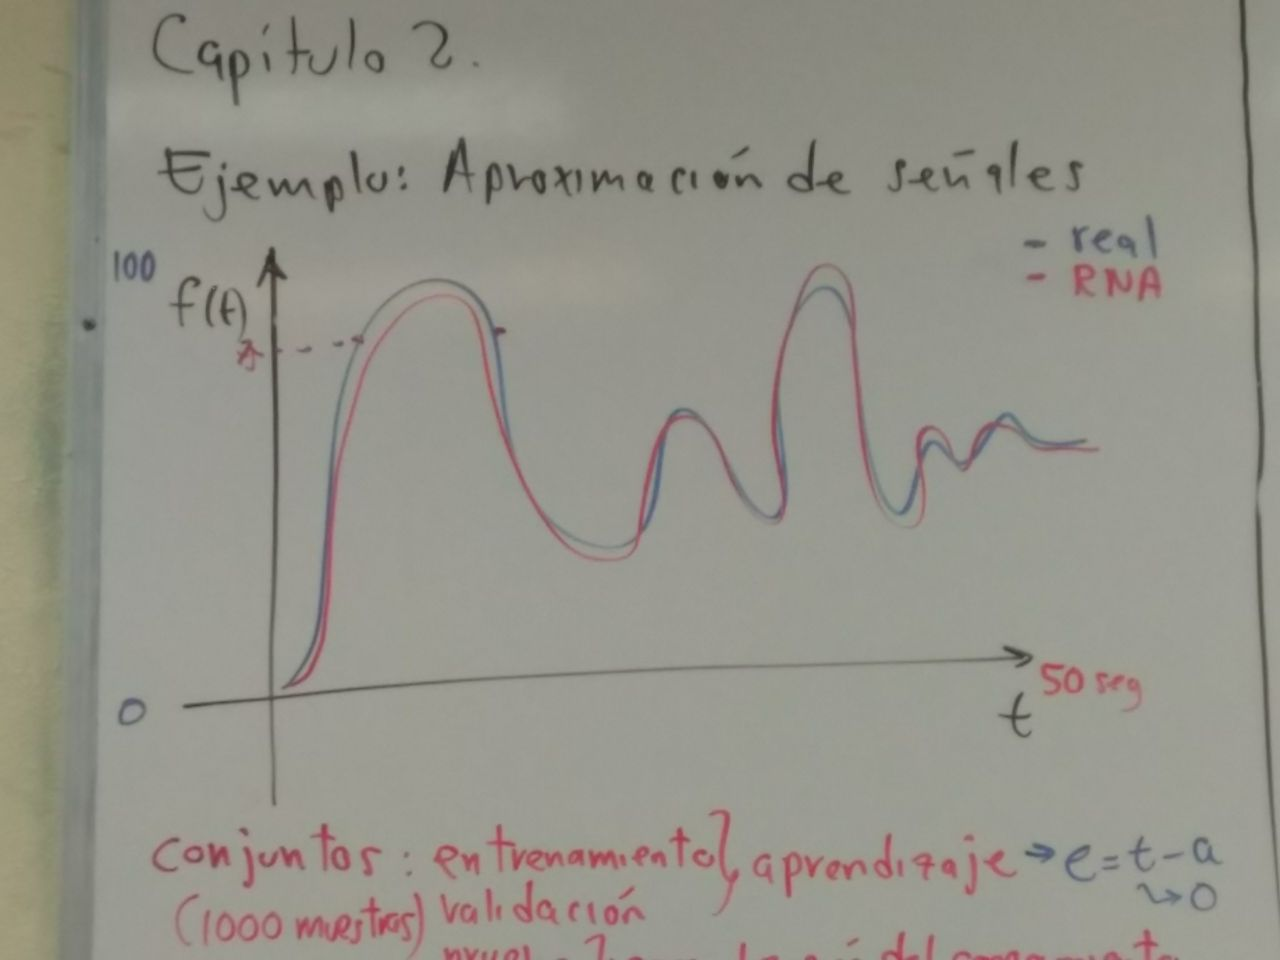
\includegraphics[scale=.2]{purelimexample}
	\caption{Ejemplo de aproximación de señales}
\end{figure}
Conjuntos: entrenamiento, aprendizaje, validación y prueba\\
Si logra interpolar bien, se dice que logró la generalización del conocimiento ya que error=t-a$\rightarrow$ 0
\subsection{Función logsigmoid}
Esta función toma como entrada n que puede tener valores entre $-\inf$ y $+\inf$; y la reduce a una salida en el rando de 0 a 1, de acuerdo a la siguiente expresión
$$a = \frac{1}{1 + e^{-n}}$$
\begin{figure}[h!]
	\centering
	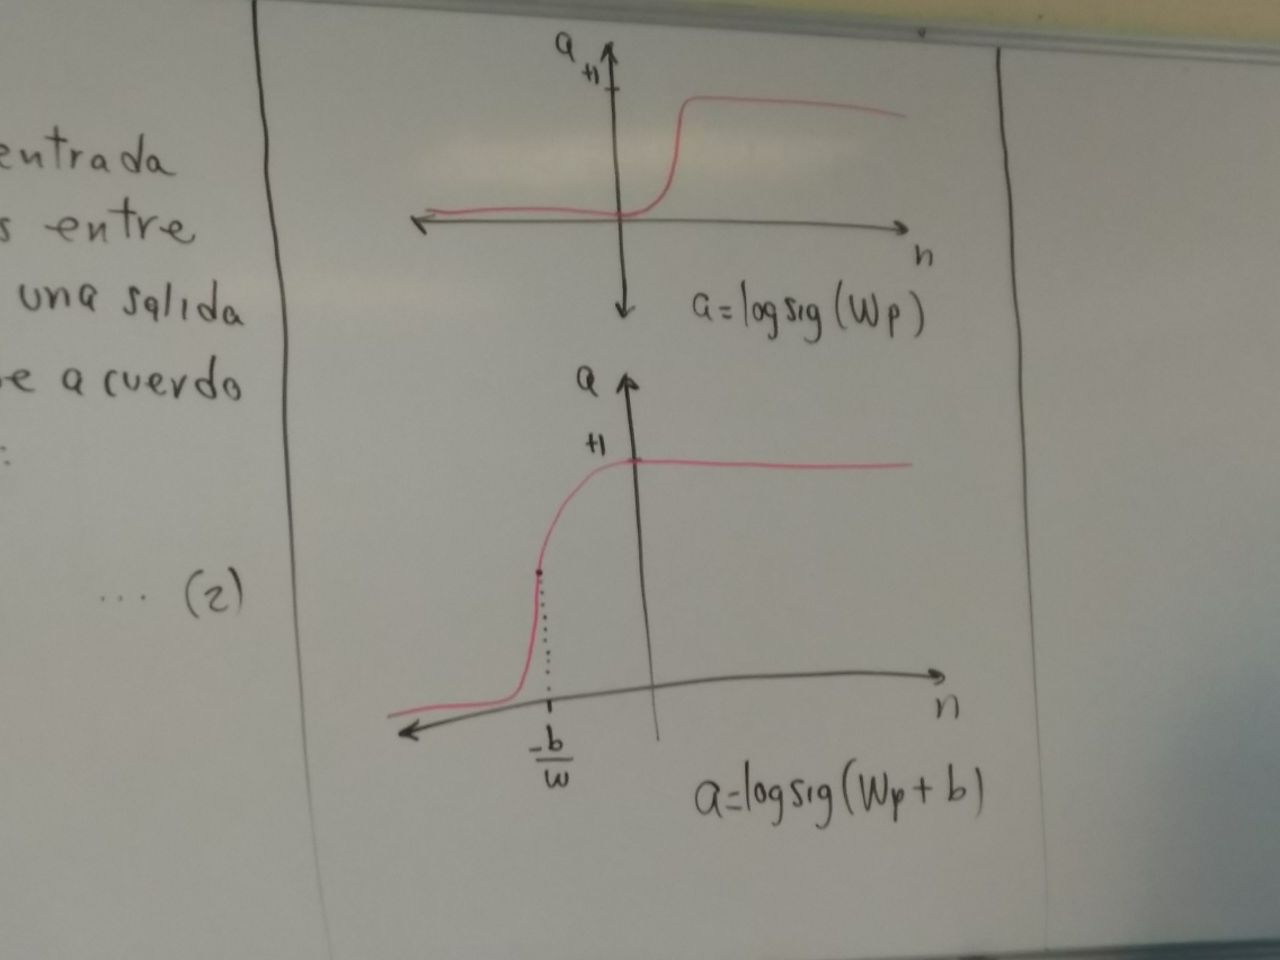
\includegraphics[scale=.2]{logsig}
	\caption{Función logsig}
\end{figure}
Esta función es usada comúnmente en redes neuronales multicapa que son entrenadas mediante el algoritmo backpropagation debdo a que esta técnica requiere que las funciones de transferencia de las capas ocultas sean no lineales, continuas y diferenciables.\\
\textbf{La linea que separa las clases se llama frontera de desición}

\section{Red Hamming}
Esta RNA fue diseñada explicitamente para resolver problemas de reconocimiento de patrones binarios (+1 o -1). Esta RNA es interesante, debido a que usa dos tipos de capas, una feed foward y otra recurrente. En hamming el mismo número de neuronas \textbf{AQUI VA UNA FOTO}\\

\subsection{Observaciones}
\begin{enumerate}
	\item El número de neuronas en ambas capas, es el mismo, s
	\item La capa recurrente no tiene bias
	\item La recurrencia se lleva a cabo usando la señal de salida $a^2(t)$ como entrada a los pesos $W^2$
\end{enumerate}

\subsection{Capa FeedForward}
Esta capa calcula la correlación o producto interno entre cada unos de los vecgores protitipo y e patrón de entrada. Con este objetivo, as filas de la matriz de pesos $W_1$, serán cada uno de los patrones prototipo.\\
Para el ejemplo de clasificar una fruta en manzanas y naranjas, la matriz queda como:

\[
W^1 = 
\begin{bmatrix}
	p_1^t\\
	p_2^t
\end{bmatrix}
=
\begin{bmatrix}
+1 & -1 &- 1 \\
+1 & +1 & -1
\end{bmatrix}
\]
\textbf{Nota: Naraja es el primer renglón y manzana el segundo}\\
El valor del bias,$b^1$ es igual a R. Para nuestro ejemplo:\\
donde $S = 2$, ya que es igual al número de patrones prototipo. \textbf{Nota: Al agregar el valor R, se garantiza que las salidas de esta capa no sean negativas, lo cual es necesario para el correcto funcionamiento de la capa recurrente}

\subsection{Capa Recurrente}
Las neuronas de esta capa se inicializan con las salidas de la capa feed foward. En esta capa las neuronas compiten entre ellas para determinar a la ganadora.\\ Al final de la competencia, solo una neuronas de esta capa tendrás un valor diferente de cero.\\\\
La neurona ganadora indica a que clase pertence el vector de entrada. Las ecuaciones que describen esta capa son:
$$ a^2(0) = a^1$$
$$ a^2(t + 1) = poslin(W^2a^2(t)) $$
La matriz de pesos tiene la siguiente forma para el ejemplo:
\[
W^2 = 
\begin{bmatrix}
1 & - \epsilon\\
-\epsilon & 1
\end{bmatrix}
\]

donde:\\
$\epsilon$ es un valor menor a $\frac{1}{S - 1}$\\
S: es el número de neuronas en la capa recurrente\\

Para nuestro ejemplo, una iteración de la capa recurrente, se lleva a cabo con la siguiente ecuación:\\

\[
a^2(t + 1) = poslin
(\begin{bmatrix}
1 & - \epsilon\\
-\epsilon & 1
\end{bmatrix}
\begin{bmatrix}
a_1^2(t)\\
a_2^2(t)
\end{bmatrix})
\]

Esta capa seguirá realizando iteraciones hasta que converja a una solución donde una sola de las neuronas tenga un valor diferente de cero y se reputa en dos iteraciones consecutivas.\\

\subsection{Solución al problema de clasificación}
Indique a que clase pertenece el siguiente vector de entrada usando la red de hamming\\

\[
p =
\begin{bmatrix}
-1 \\
-1\\
-1
\end{bmatrix}
\]
Comenzamos calculando la capa feed foward esto se hace sollo una vez:\\
$$ a^1 = W^1p + b^1 $$\\

\[
a^1 =
\begin{bmatrix}
+1 &  - 1& -1\\
+1 &  + 1& -1
\end{bmatrix}
\begin{bmatrix}
-1 \\
-1 \\
-1
\end{bmatrix}
+
\begin{bmatrix}
3 \\
3 
\end{bmatrix}
=
\begin{bmatrix}
4 \\
2 
\end{bmatrix}
\]

Ahora se pasa a la capa de recurrente

$$ 0 < \epsilon < \frac{1}{S - 1} = 1 $$\\
Se propone $\epsilon$ = 0.5\\
Se realza la primera iteración
t = 0 $\rightarrow a^2(0) = a^1 = $  
\end{document}
